\section{Expanded fixed-backbone controls and magnitude-scaled inhibition}

\label{sec:s04-expanded}

The original S04 completed campaign expands the fixed-seed control matrix and evaluates magnitude-scaled immigrant-only and total-intensity inhibition (LI+). The earlier eight examples above remain historical results under their original numerical procedure. The expanded results below use the same declared generating regimes and shared fixed background/excitation inputs; they are not full joint nuisance refits.

The original S04 positive-control histories are generated by the original unit-mark, immigrant-only LI law. Magnitude-scaled LI+ and total-intensity attenuation are alternative fitted procedures on those same histories, not their matched generating models. Their contrast therefore measures performance under that specified generator; it does not establish relative power when magnitude-scaled or total-intensity inhibition generates the data.

The original S04 expanded roster contains 80 distinct histories, 20 in each regime, with five paired procedure/gate combinations and 400 score rows. The stress field is
\[
G_+(t,z)=\sum_{t_j<t}\exp\{\gamma Q_j-(t-t_j)/\psi\}
 \left(1+\|z-z_j\|^2/\ell^2\right)^{-2},\qquad
\gamma=\tfrac34\log 10.
\]
Here $Q_j$ is excess magnitude, so the reference excess is zero. Original LI uses the same field with unit magnitude weights. This bounded design retains a common shadow radius; it does not fit a magnitude-dependent rupture radius. With the shared fixed backbone written $B+nH$, the two LI+ intensities are
\[
 \lambda_{\rm imm}=B e^{-\eta G_+}+nH,
 \qquad \lambda_{\rm total}=(B+nH)e^{-\eta G_+}.
\]
The gate retains an active fit only when its training log-likelihood improvement exceeds $\tfrac32\log N_{\rm train}$.

The BIC-style gate is a training-only complexity penalty, not a Davies-calibrated test or a nominal-size guarantee. The gate can select the exact uninhibited floor. A held-out win and an active training fit are distinct outcomes. No seed was redrawn and no negative score was removed.

\begingroup\footnotesize\setlength{\tabcolsep}{3pt}

\begin{longtable}{@{}llrrrrr@{}}

\toprule Regime & Procedure & $N$ & Mean gain & MC SE & Median & Wins \\

\midrule\endfirsthead

\toprule Regime & Procedure & $N$ & Mean gain & MC SE & Median & Wins \\

\midrule\endhead

\bottomrule\endlastfoot

Uniform null & LI & 20 & -2.9299 & 0.9259 & -1.6435 & 3 \\

Uniform null & LI+ immigrant gated & 20 & 0.0000 & 0.0000 & 0.0000 & 0 \\

Uniform null & LI+ immigrant & 20 & -2.9514 & 1.3451 & -0.3835 & 4 \\

Uniform null & LI+ total gated & 20 & 0.0000 & 0.0000 & 0.0000 & 0 \\

Uniform null & LI+ total & 20 & -74.6499 & 42.9783 & -2.2181 & 1 \\

Smooth null & LI & 20 & -3.4230 & 1.3263 & -2.2716 & 4 \\

Smooth null & LI+ immigrant gated & 20 & 0.0000 & 0.0000 & 0.0000 & 0 \\

Smooth null & LI+ immigrant & 20 & -3.6408 & 1.5156 & -1.9787 & 4 \\

Smooth null & LI+ total gated & 20 & 0.0000 & 0.0000 & 0.0000 & 0 \\

Smooth null & LI+ total & 20 & -448.5272 & 445.0217 & -0.0604 & 3 \\

Narrow/short & LI & 20 & -3.8713 & 1.3147 & -2.3528 & 3 \\

Narrow/short & LI+ immigrant gated & 20 & 0.0000 & 0.0000 & 0.0000 & 0 \\

Narrow/short & LI+ immigrant & 20 & -3.4720 & 1.6063 & -1.1309 & 4 \\

Narrow/short & LI+ total gated & 20 & 0.0000 & 0.0000 & 0.0000 & 0 \\

Narrow/short & LI+ total & 20 & -129.3344 & 103.6071 & -0.6334 & 6 \\

Broad/long & LI & 20 & 33.8922 & 1.2083 & 33.4049 & 20 \\

Broad/long & LI+ immigrant gated & 20 & 28.3296 & 1.6682 & 26.6651 & 20 \\

Broad/long & LI+ immigrant & 20 & 28.3296 & 1.6682 & 26.6651 & 20 \\

Broad/long & LI+ total gated & 20 & -5.4013 & 13.7572 & 3.9231 & 10 \\

Broad/long & LI+ total & 20 & -5.3446 & 13.7585 & 4.4063 & 14 \\

\end{longtable}\endgroup

Mean and median gains are total held-out log-score differences from the shared uninhibited baseline; MC SE is the sample standard deviation divided by the square root of the number of independent seeded datasets within each regime. It is a descriptive finite-sample summary, not a calibrated confidence interval. The unbounded magnitude transforms and large retained losses do not by themselves establish finite score variance or a Gaussian approximation. The broad/long regime supports improved mean performance for original LI and immigrant-only LI+. Total-intensity attenuation has a negative mean even there, despite a positive median. The large negative means in other regimes are retained rather than trimmed.

In original S04, gating selects the uninhibited floor throughout both null regimes, but also throughout the narrow/short positive regime. This demonstrates the sensitivity--overfitting tradeoff of this procedure on these controls; it does not establish nominal Type I error or general detection power.

The original S04 completed matrix combines accepted first-pass results with quadrature refinement and same-history finer-grid refits. Training-only selection preserves the prescribed starts, bounds and exact uninhibited floor. Finer-grid validation checks retained candidates, score decomposition and forecast spread. Independent compiled CPU replays cover predeclared anchors; the remaining cases have per-case numerical checks and sampled-audit coverage, not individual independent replay. All aggregate tables and their source identities are retained in the evidence bundle.

These results extend the synthetic evidence only. They do not replace the observed California comparison, for which the completed observed LI+ evaluation is reported in Section~\ref{sec:s04-observed-completed} below.

\begin{figure}[p]\centering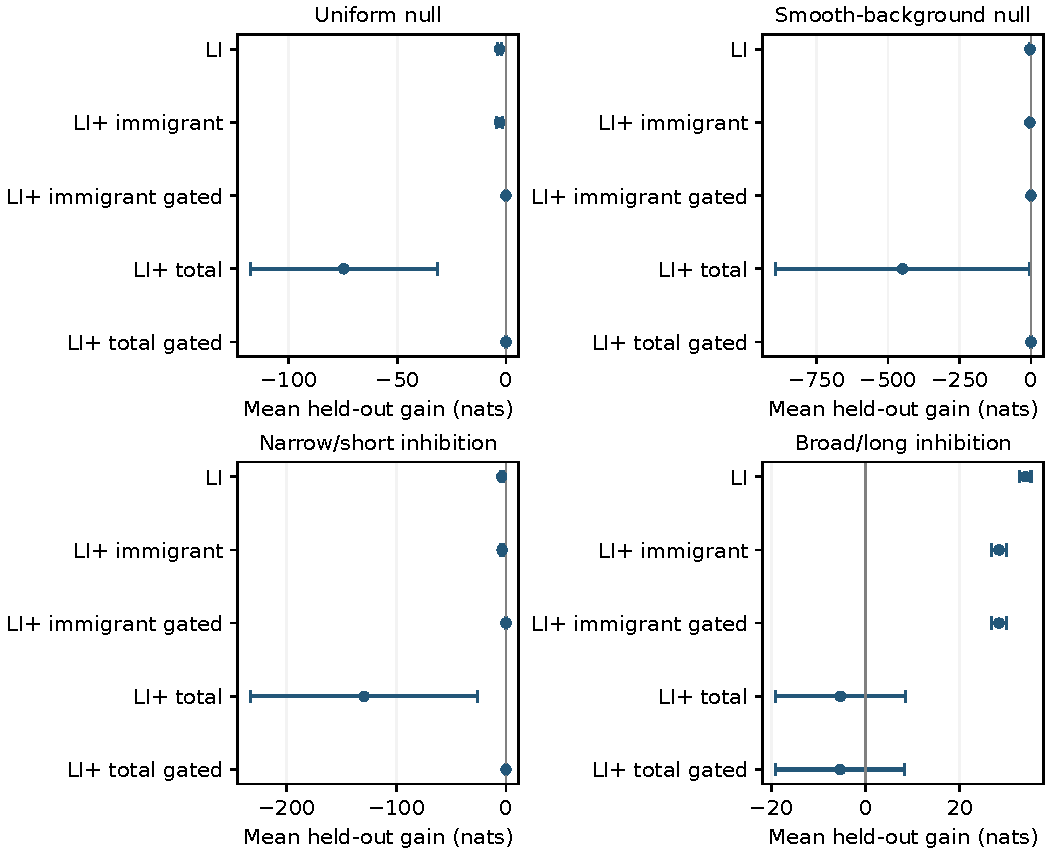
\includegraphics[width=\linewidth]{s04_unitmark_mean_gains.pdf}
\caption{Original S04 unit-mark fixed-backbone controls. Points show mean held-out gain and bars show the descriptive sample standard deviation divided by the square root of the row denominator, labelled MC SE in the table. These bars are not calibrated confidence intervals. Panels retain their full linear ranges, including large losses; horizontal scales differ. Each plotted summary uses the full corresponding row denominator in the preceding table. The zero line is the shared uninhibited comparator.}\end{figure}


\subsection{Matched magnitude-scaled generators (S04B)}

\label{sec:s04b-matched}

S04B is a separate matched-generator extension, not a replacement for the unit-mark S04 controls above. Magnitude-scaled immigrant-only and total-intensity laws each generate narrow/short and broad/long positive controls. Only accepted events enter the strictly prior stress field and spawn descendants. Immigrant-only generation thins immigrant proposals; total-intensity generation also thins offspring proposals.

The completed extension contains 80 independent seeded histories and 400 paired procedure scores. Every regime--procedure row has 20 histories. The five procedures share each history and are not independent replications. The original null histories remain valid at zero inhibition; they are not regenerated or added to this positive-control denominator.

Generation uses the smooth background and the same day-based split as the original controls: warmup $[0, 30)$, training $[30, 395)$ and test $[395, 760)$, with horizon $760$ days. For each generating law, narrow/short inhibition has $(\eta,\ell,\psi)=(0.5,5\ {\rm km},1/24\ {\rm day})$ and broad/long inhibition has $(2.0,50\ {\rm km},30\ {\rm days})$. The magnitude scaling and the two intensity definitions are those displayed above. Seeds are predeclared and retained without replacement: immigrant narrow/short $410401$ through $410420$, immigrant broad/long $410501$ through $410520$, total narrow/short $410601$ through $410620$, and total broad/long $410701$ through $410720$. Training uses all $8$ prescribed starts plus the exact uninhibited floor at quadrature order $16$; every retained finite state is checked at order $32$ on training and test windows. The first seed in each regime is the predeclared independent CPU anchor. These settings and source identities are retained in the bundled frozen-method projection and protocol.

All fits hold the shared background and excitation backbone fixed. Training-only selection and the complexity gate retain the exact uninhibited floor. Full saved-row arithmetic and numerical gates are audited; independent CPU objective and gradient replays cover 48 predeclared phase--model contexts from the anchor histories, rather than every history.

Under immigrant: narrow/short generation, the matched raw procedure has a negative mean gain and a negative median; its gated version has a negative mean. Under immigrant: broad/long generation, the matched raw procedure has a positive mean gain and a positive median; its gated version has a positive mean. Under total: narrow/short generation, the matched raw procedure has a negative mean gain and a negative median; its gated version has a positive mean. Under total: broad/long generation, the matched raw procedure has a positive mean gain and a positive median; its gated version has a positive mean. Both matched raw procedures lose on average in their narrow/short settings. The positive gated mean under narrow/short total generation comes from a single winning active history and otherwise exact-floor ties; it does not demonstrate reliable recovery. Under narrow/short immigrant generation, the matched gate instead retains a single active loss and otherwise floor ties. In both broad/long generating settings, matched raw and gated procedures win on every history in this declared bank. These outcomes remain conditional on the fixed nuisance backbone and chosen regimes.

Mean and median gains below are total held-out log-score differences per simulated history, not per earthquake. MC SE is the within-regime sample standard deviation divided by the square root of the history denominator. It is descriptive: these heavy-tailed marked laws do not supply an automatic finite-variance or Gaussian guarantee. Wilson intervals describe bounded held-out-win indicators under the declared seeded simulation design; they are not intervals for the mean gain or calibrated detection power. A positive held-out gain, an active fit and an identified physical mechanism are different statements.

\begingroup\footnotesize\setlength{\tabcolsep}{3pt}

\begin{longtable}{@{}lrrrrrrr@{}}

\caption{S04B: Immigrant: narrow/short. Wins are strict positive gains; interval endpoints are probabilities.}\label{tab:s04b-4}\\

\toprule Procedure & $N$ & Mean & MC SE & Median & Wins & Wilson 95\% & Active \\

\midrule\endfirsthead

\toprule Procedure & $N$ & Mean & MC SE & Median & Wins & Wilson 95\% & Active \\

\midrule\endhead

\bottomrule\endlastfoot

LI & 20 & -3.9493 & 1.2142 & -2.7555 & 2 & [0.028, 0.301] & 19 \\

LI+ immigrant & 20 & -4.5674 & 1.6218 & -2.0582 & 5 & [0.112, 0.469] & 20 \\

LI+ immigrant gated & 20 & -1.3440 & 1.3440 & 0.0000 & 0 & [0.000, 0.161] & 1 \\

LI+ total & 20 & -21.5766 & 9.8329 & -3.1228 & 4 & [0.081, 0.416] & 19 \\

LI+ total gated & 20 & -1.0043 & 1.0043 & 0.0000 & 0 & [0.000, 0.161] & 1 \\

\end{longtable}\endgroup

\begingroup\footnotesize\setlength{\tabcolsep}{3pt}

\begin{longtable}{@{}lrrrrrrr@{}}

\caption{S04B: Immigrant: broad/long. Wins are strict positive gains; interval endpoints are probabilities.}\label{tab:s04b-5}\\

\toprule Procedure & $N$ & Mean & MC SE & Median & Wins & Wilson 95\% & Active \\

\midrule\endfirsthead

\toprule Procedure & $N$ & Mean & MC SE & Median & Wins & Wilson 95\% & Active \\

\midrule\endhead

\bottomrule\endlastfoot

LI & 20 & 44.3122 & 1.4559 & 43.3861 & 20 & [0.839, 1.000] & 20 \\

LI+ immigrant & 20 & 48.3868 & 0.9599 & 47.7879 & 20 & [0.839, 1.000] & 20 \\

LI+ immigrant gated & 20 & 48.3868 & 0.9599 & 47.7879 & 20 & [0.839, 1.000] & 20 \\

LI+ total & 20 & 19.4993 & 7.2001 & 35.3378 & 15 & [0.531, 0.888] & 19 \\

LI+ total gated & 20 & 19.3802 & 7.2159 & 35.3378 & 14 & [0.481, 0.855] & 18 \\

\end{longtable}\endgroup

\begingroup\footnotesize\setlength{\tabcolsep}{3pt}

\begin{longtable}{@{}lrrrrrrr@{}}

\caption{S04B: Total: narrow/short. Wins are strict positive gains; interval endpoints are probabilities.}\label{tab:s04b-6}\\

\toprule Procedure & $N$ & Mean & MC SE & Median & Wins & Wilson 95\% & Active \\

\midrule\endfirsthead

\toprule Procedure & $N$ & Mean & MC SE & Median & Wins & Wilson 95\% & Active \\

\midrule\endhead

\bottomrule\endlastfoot

LI & 20 & -1.7818 & 0.6357 & -0.9047 & 5 & [0.112, 0.469] & 20 \\

LI+ immigrant & 20 & -3.2420 & 1.2527 & -0.5371 & 7 & [0.181, 0.567] & 20 \\

LI+ immigrant gated & 20 & 0.0000 & 0.0000 & 0.0000 & 0 & [0.000, 0.161] & 0 \\

LI+ total & 20 & -14.5947 & 7.8248 & -0.1064 & 10 & [0.299, 0.701] & 20 \\

LI+ total gated & 20 & 0.0686 & 0.0686 & 0.0000 & 1 & [0.009, 0.236] & 1 \\

\end{longtable}\endgroup

\clearpage

\begingroup\footnotesize\setlength{\tabcolsep}{3pt}

\begin{longtable}{@{}lrrrrrrr@{}}

\caption{S04B: Total: broad/long. Wins are strict positive gains; interval endpoints are probabilities.}\label{tab:s04b-7}\\

\toprule Procedure & $N$ & Mean & MC SE & Median & Wins & Wilson 95\% & Active \\

\midrule\endfirsthead

\toprule Procedure & $N$ & Mean & MC SE & Median & Wins & Wilson 95\% & Active \\

\midrule\endhead

\bottomrule\endlastfoot

LI & 20 & 42.5503 & 1.7274 & 44.8818 & 20 & [0.839, 1.000] & 20 \\

LI+ immigrant & 20 & 49.2902 & 1.3502 & 48.5828 & 20 & [0.839, 1.000] & 20 \\

LI+ immigrant gated & 20 & 49.2902 & 1.3502 & 48.5828 & 20 & [0.839, 1.000] & 20 \\

LI+ total & 20 & 53.2332 & 2.1250 & 51.2906 & 20 & [0.839, 1.000] & 20 \\

LI+ total gated & 20 & 53.2332 & 2.1250 & 51.2906 & 20 & [0.839, 1.000] & 20 \\

\end{longtable}\endgroup

Active counts record off-floor selection ($\hat\eta > 0$), including the effect of the training-only gate. The bundled public audit exports score contrasts and off-floor indicators rather than empirical distributions of selected $(\hat\eta,\hat\ell,\hat\psi)$: S04B evaluates held-out predictive log-score gain rather than parameter recovery. An active fit can still overfit or adjust shared coordinates without recovering the generating $(\eta,\ell,\psi)$. Zero gains remain ties, not wins. No negative gain is trimmed and no seed is substituted. The completed matched generation resolves the prior generating-law gap for these bounded settings; it does not resolve joint nuisance estimation, nominal test size, general recovery or prospective observational evidence.

\begin{figure}[p]\centering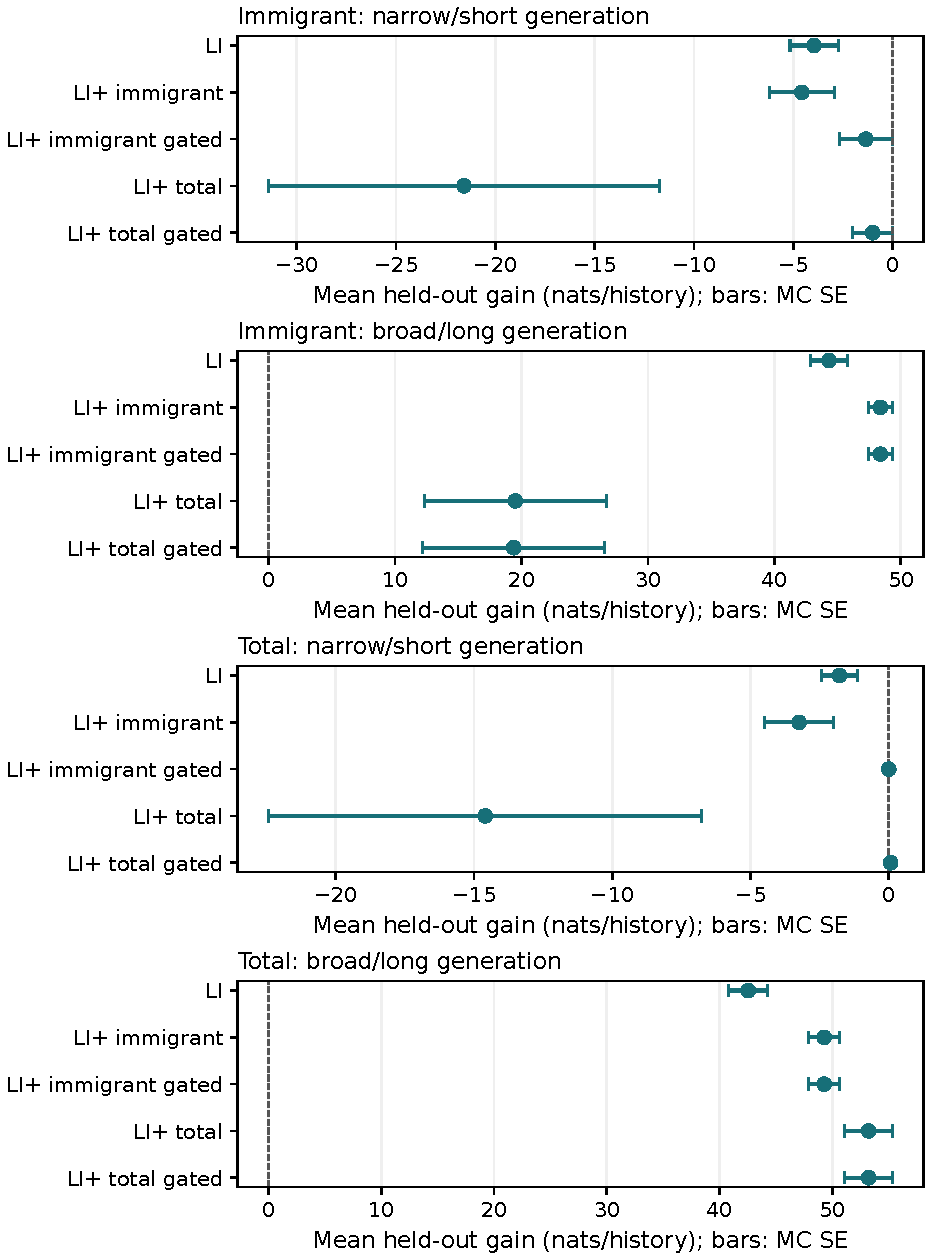
\includegraphics[width=\linewidth]{s04_expanded_mean_gains.pdf}

\caption{S04B matched-generator controls. Each panel keeps its own full linear range. Points show row means; bars show descriptive MC SE, not calibrated confidence intervals. Each procedure uses the same complete history denominator within its generating regime. The dashed zero line denotes the uninhibited floor; regimes are not pooled.}\label{fig:s04b-matched}\end{figure}
